%%%%%%%%%%%%%%%%%%%%%%%%%%%%%%%%%%%%%%%%%
% Short Sectioned Assignment LaTeX Template Version 1.0 (5/5/12)
% This template has been downloaded from: http://www.LaTeXTemplates.com
% Original author:  Frits Wenneker (http://www.howtotex.com)
% License: CC BY-NC-SA 3.0 (http://creativecommons.org/licenses/by-nc-sa/3.0/)
%%%%%%%%%%%%%%%%%%%%%%%%%%%%%%%%%%%%%%%%%

%----------------------------------------------------------------------------------------
%	PACKAGES AND OTHER DOCUMENT CONFIGURATIONS
%----------------------------------------------------------------------------------------

\documentclass[paper=a4, fontsize=11pt]{scrartcl} % A4 paper and 11pt font size

% ---- Entrada y salida de texto -----

\usepackage[T1]{fontenc} % Use 8-bit encoding that has 256 glyphs
\usepackage[utf8]{inputenc}
%\usepackage{fourier} % Use the Adobe Utopia font for the document - comment this line to return to the LaTeX default

\usepackage{xcolor}
\usepackage{fancyhdr}
\usepackage{listings, lstautogobble}
\usepackage{comment}

\usepackage{subfigure} % subfiguras

%----------
\lstdefinestyle{customc}{
	belowcaptionskip=1\baselineskip,
	autogobble=true,
	breaklines=true,
	frame=L,
	xleftmargin=\parindent,
	language=C,
	showstringspaces=false,
	basicstyle=\footnotesize\ttfamily,
	keywordstyle=\bfseries\color{green!40!black},
	commentstyle=\itshape\color{purple!40!black},
	identifierstyle=\color{blue},
	stringstyle=\color{orange},
}

\lstdefinestyle{bashmc}{
	frame=l,
	tabsize=2,
	breaklines=true,
	xleftmargin=\parindent,
	basicstyle=\ttfamily,
	showstringspaces=false,
	commentstyle=\color{red},
	keywordstyle=\color{blue},
	autogobble=true,
}





% ---- Idioma --------

\usepackage[spanish, es-tabla]{babel} % Selecciona el español para palabras introducidas automáticamente, p.ej. "septiembre" en la fecha y especifica que se use la palabra Tabla en vez de Cuadro

% ---- Otros paquetes ----
\usepackage{eurosym} % para el euro
\usepackage{url} % ,href} %para incluir URLs e hipervínculos dentro del texto (aunque hay que instalar href)
\usepackage{amsmath,amsfonts,amsthm} % Math packages
\usepackage{centernot}
%\usepackage{graphics,graphicx, floatrow} %para incluir imágenes y notas en las imágenes
\usepackage{graphics,graphicx, float} %para incluir imágenes y colocarlas

% Para hacer tablas comlejas
%\usepackage{multirow}
%\usepackage{threeparttable}

%\usepackage{sectsty} % Allows customizing section commands
%\allsectionsfont{\centering \normalfont\scshape} % Make all sections centered, the default font and small caps

\usepackage{fancyhdr} % Custom headers and footers
\pagestyle{fancyplain} % Makes all pages in the document conform to the custom headers and footers
\fancyhead{} % No page header - if you want one, create it in the same way as the footers below
\fancyfoot[L]{} % Empty left footer
\fancyfoot[C]{} % Empty center footer
\fancyfoot[R]{\thepage} % Page numbering for right footer
\renewcommand{\headrulewidth}{0pt} % Remove header underlines
\renewcommand{\footrulewidth}{0pt} % Remove footer underlines
\setlength{\headheight}{13.6pt} % Customize the height of the header

\numberwithin{equation}{section} % Number equations within sections (i.e. 1.1, 1.2, 2.1, 2.2 instead of 1, 2, 3, 4)
\numberwithin{figure}{section} % Number figures within sections (i.e. 1.1, 1.2, 2.1, 2.2 instead of 1, 2, 3, 4)
\numberwithin{table}{section} % Number tables within sections (i.e. 1.1, 1.2, 2.1, 2.2 instead of 1, 2, 3, 4)

\setlength\parindent{0pt} % Removes all indentation from paragraphs - comment this line for an assignment with lots of text

\newcommand{\horrule}[1]{\rule{\linewidth}{#1}} % Create horizontal rule command with 1 argument of height


%----------------------------------------------------------------------------------------
%	TÍTULO Y DATOS DEL ALUMNO
%----------------------------------------------------------------------------------------

\title{	
\normalfont \normalsize 
\textsc{\textbf{Curso 2016-2017} \\ Grado en Ingeniería Informática \\ Universidad de Granada} \\ [25pt] % Your university, school and/or department name(s)
\horrule{0.5pt} \\[0.4cm] % Thin top horizontal rule
\huge Memoria descriptiva de la propuesta de museo \\ % The assignment title
\horrule{2pt} \\[0.5cm] % Thick bottom horizontal rule
}

\author{Samuel Cardenete Rodríguez \\
	Juan Ramón Gómez Berzosa\\
	Arthur Mickael Rodríguez Nesterenko\\
	Carlos Manuel Sequí Sánchez} % Nombre y apellidos

\date{\normalsize\today} % Incluye la fecha actual

%----------------------------------------------------------------------------------------
% DOCUMENTO
%----------------------------------------------------------------------------------------

\begin{document}

\maketitle % Muestra el Título

\newpage %inserta un salto de página

\tableofcontents % para generar el índice de contenidos

\newpage

\section{Descripción de la idea del museo}

Nuestro museo será una habitación lo suficientemente grande formada por una serie de estructuras (como puestos de un mercadillo, vitrinas...) vacías, es decir, sin objetos físicos, pero con etiquetas idetificativas mediante las cuales mostraremos al usuario el contenido del museo de manera virtual. \\
La idea es que cuando entremos al museo nos pongamos unas gafas de realidad aumentada (las cuales permitirán generar una ambientación virtual realizando una simbiosis entre esta y el propio espacio físico del museo) y que la primera interacción con ellas sea seleccionar la época en la que queremos ambientar la sala ( Antigua Roma, medievo, prehistoria, edad contemporánea…). En función de esta elección nuestra sala se ambientará en una época u otra, de modo que  si elegimos la antigua Roma por ejemplo, las estructuras del museo serán reconvertidas por las gafas en puestos de un mercado de la época romana. En dicho mercado habrán puestos y vitrinas con varias etiquetas identificativas, las cuales se encargarán de mostrar distintos elementos o productos que podían encontrarse en dicha época/lugar, como por ejemplo jarrones de la época, especias de la época, alimentos... También habrá repartidas por la escena monumentos o edificios de la época, así como varios personajes (identificables mediante etiquetas), como el césar, un romano, un mercader con los que se podrá conversar acerca de la temática del museo en esa época… \\
A parte del mercado, habrá una pantalla controlada mediante una interfaz gestual que nos permitirá observar e informarnos de las armas de la época en la que nos encontremos ambientados.\\
Esta gestión del museo, es decir, el uso de gafas de realidad aumentada y las etiquetas identificativas, permitirá que varios usuarios en el mismo museo puedan acceder a distintas épocas sin molestarse los unos a los otros, ni tener que guardar colas o esperarse entre ellos para interaccionar con las distintas partes del museo.
\\
En definitiva, vamos a dar un salto intentando romper con lo cotidiano y la monotonía actual existente en los museos, pretendiendo ir más allá con la oferta de visitas a distintos museos desde la misma sala y haciendo llegar las comodidades de la tecnología a personas que tengan más dificultades que otras en las visitas turísticas.\\  

El proyecto de la asignatura se basa en adaptar una serie de interfaces para poder utilizarlas en el museo que hemos planteado. Las interfaces a utilizar son:

\begin{itemize}
	\item Interfaz oral.
	\item Interfaz sensorial por móvil.
	\item Interfaz gestual.
\end{itemize}

A continuación procedemos a describirlas individualmente de forma detallada.

\newpage

\section{Interfaz oral}

Una vez elegida la época en la que queremos explorar el museo, nos encontraremos distintos personajes repartidos por la sala que sean característicos de la época (o la zona). La idea es que cuando nos acerquemos a un personaje específico, acerquemos nuestro dispositivo móvil y mediante el uso de etiquetas NFC nos reconozca al personaje. Una vez reconocido, podremos entablar una conversación con el personaje seleccionado de modo que podamos preguntarle por información relativa a su identidad, a la época de donde viene, de su trabajo... etc y además nos permitirá valorar nuestra experiencia en el museo, incluso aconsejarnos visitar a otros personajes de la sala que estén relacionados con su profesión.  \\ 

Una gran ventaja de nuestra propuesta de museo es que al darle la posibilidad a cada usuario distinto que entre en la sala explorar sobre una época u otra, también le da la posibilidad a distintos usuarios de interactuar con distintos personajes aunque ambos estén en la misma sala y se hayan acercado a la misma etiqueta. Esto es posible porque las etiquetas mostrarán distintos personajes en función de la época elegida por cada turista del museo. \\ 

Una ventaja más de esta aplicación es que ya no tendrás que estar escuchando lo que otro turista está dialogando con un personaje, ni siquiera tener que esperar a que termine de conversar con él (a diferencia de las pantallas actuales con los personajes disponibles en el museo), ya que cada visitante tendrá la aplicación en su propio dispositivo móvil y podrán escuchar directamente las respuestas del personaje en este. Para ello la idea es que se usen auriculares, de modo que se proporcionarán auriculares al entrar para las personas que no se los traigan. Cabe destacar que hemos dado por supuesto que todas las personas dispondrán de un dispositivo móvil, ya que la propia época actual casi que lo requiere, aunque aún así se prestarán dispositivos móviles durante la visita del museo para aquellas personas que no dispongan de batería, que no tengan dispositivo móvil, que estén pendientes de alguna llamada urgente... etc. \\

Otro apartado que cabe destacar, es que una vez que el usuario se haya acercado a un personaje, esta elección se guardará en la aplicación hasta que se acerque a otro personaje, de modo que así pueda ir caminando por el museo el visitante observando más cosas mientras está dialogando con este. También, aunque lo normal sea que nos acerquemos al personaje, también podremos seleccionar mediante un menú disponible en nuestra aplicación a los distintos personajes, especialmente por personas con movilidad reducida que no puedan estar paseándose por la sala o simplemente para personas que no les apetezca recorrerse todo el museo para hablar con un determinado personaje. \\

La aplicación tendrá un campo de texto que almacenará las respuestas del personaje, de modo que las personas que sean sordas puedan también mantener un diálogo con el personaje o simplemente que cualquier persona que no haya entendido al personaje pueda leer su respuesta detenidamente. También se podrán seleccionar distintos idiomas para la conversación, de modo que cualquier visitante del muso pueda disponer de la información en su lenguaje natural. \\

En definitiva, tendremos una aplicación muy funcional, ya que permitirá interactuar con distintos personajes sin tener que tener pantallas gigantes por el museo dedicadas a esto y tener que estar esperando para dialogar con estos, y simple, ya que cualquier persona que esté más experimentada o menos en el uso de las tecnologías podrá utilizarla.

\subsection{Procesador de lenguaje natural - DialogFlow}

A la hora de elegir el procesador de lenguaje natural hemos decidido utilizar Dialog Flow.\\ 

El SDK de Android API.AI facilita la integración del reconocimiento de voz con la API de procesamiento de lenguaje natural DialogFlow en dispositivos Android. El módulo permite usar comandos de voz e integración con escenarios de diálogo definidos para un agente particular de DialogFlow. \cite{git}\\

DialogFlow ofrece a los usuarios una nueva forma de interactuar con su producto mediante la construcción de interfaces de voz conversacionales basadas en texto impulsados por inteligencia artificial. \\

El proceso que un agente de Dialogflow sigue desde la invocación hasta la realización (respuesta) es parecido a responder a alguien una pregunta. \\ 
Cuando un usuario hace una petición al servicio, se genera un intento que el agente de DialogFlow interpreta para analizar la información del usuario y responder a sus peticiones. De este modo, para que el agente entienda la pregunta (el intento) será necesario indicarle como la misma pregunta se puede hacer de distintas formas, así que cuantas más formas se especifiquen mejor entenderá el agente al usuario. Finalmente, cuando procese la respuesta se la devolverá al usuario.\\

También cabe destacar que el agente necesita saber que información es relevante para el usuario, por ello se utilizarán entidades. De este modo podremos quedarnos con información relevante para responder en otras preguntas (usando los contextos), responder a la misma pregunta que nos ha realizado utilizando dicha información o incluso utilizarlas para detectar palabras claves para la conversación. \\

Como hemos mencionado, también es necesario a veces que el agente almacene información relativa a respuestas anteriores para poder dar respuestas personalizadas para las siguientes preguntas, para ello, usaremos los contextos. Estos contextos sirven para poder utilizar dicha información para las respuestas mientras estén activos, continuar conversaciones que habían sido interrumpidas por errores del sistema o del usuario, mantener un diálogo no lineal con el agente... etc. \\

Para poder establecer diálogos lineales se pueden usar los promts, mediante los cuales podemos definir que una entidad tenga que aparecer sí o sí en una pregunta del usuario y darle una respuesta personalizada si le falta dicha entidad, es decir, obligar a que el usuario incluya la entidad en su pregunta ya que puede ser relevante para la respuesta del agente. \\ 

Una vez explicado el procesador de lenguaje que vamos a utilizar y algunas de sus funciones que utilizaremos, pasaremos a describir las preguntas que hemos configurado para nuestro agente indicando que funcionalidades hemos usado de DialogFlow para implementar los diálogos. \\

Todas las definiciones han sido conseguidas de: \cite{dialogo}.
\subsection{Preguntas disponibles}
A la hora de la implementación, como hemos decidido hacer compatible nuestra aplicación con distintos idiomas, hemos creado un agente de DialogFlow específico para cada idioma. En nuestro caso solo hemos creado un agente en inglés y otro en español. Para simplificar la explicación, comentaremos el funcionamiento del agente  en español ya que el otro es exactamente igual pero con las entidades e intentos (y respuestas) traducidos a inglés. \\

Las preguntas disponibles serán:

\subsubsection{Bienvenida}

A la hora de la bienvenida tenemos que dirigirnos al agente utilizando saludos formales, construidos con buenos días (tardes, noches) y especificando la palabra señor, ya que si no detecta la palabra señor saltará un prompt que exigirá al usuario que la pregunta tenga dicha palabra. Tanto buenos días (como sus derivados) como señor serán dos entidades distintas, de modo que cualquier saludo similar sea válido pero sólo si esta acompañado por la palabra señor. Por tanto podremos decirle cosas del tipo: ¡Buenos días señor cooperativista!. \\

\begin{figure}[H] %con el [H] le obligamos a situar aquí la figura
	\centering
	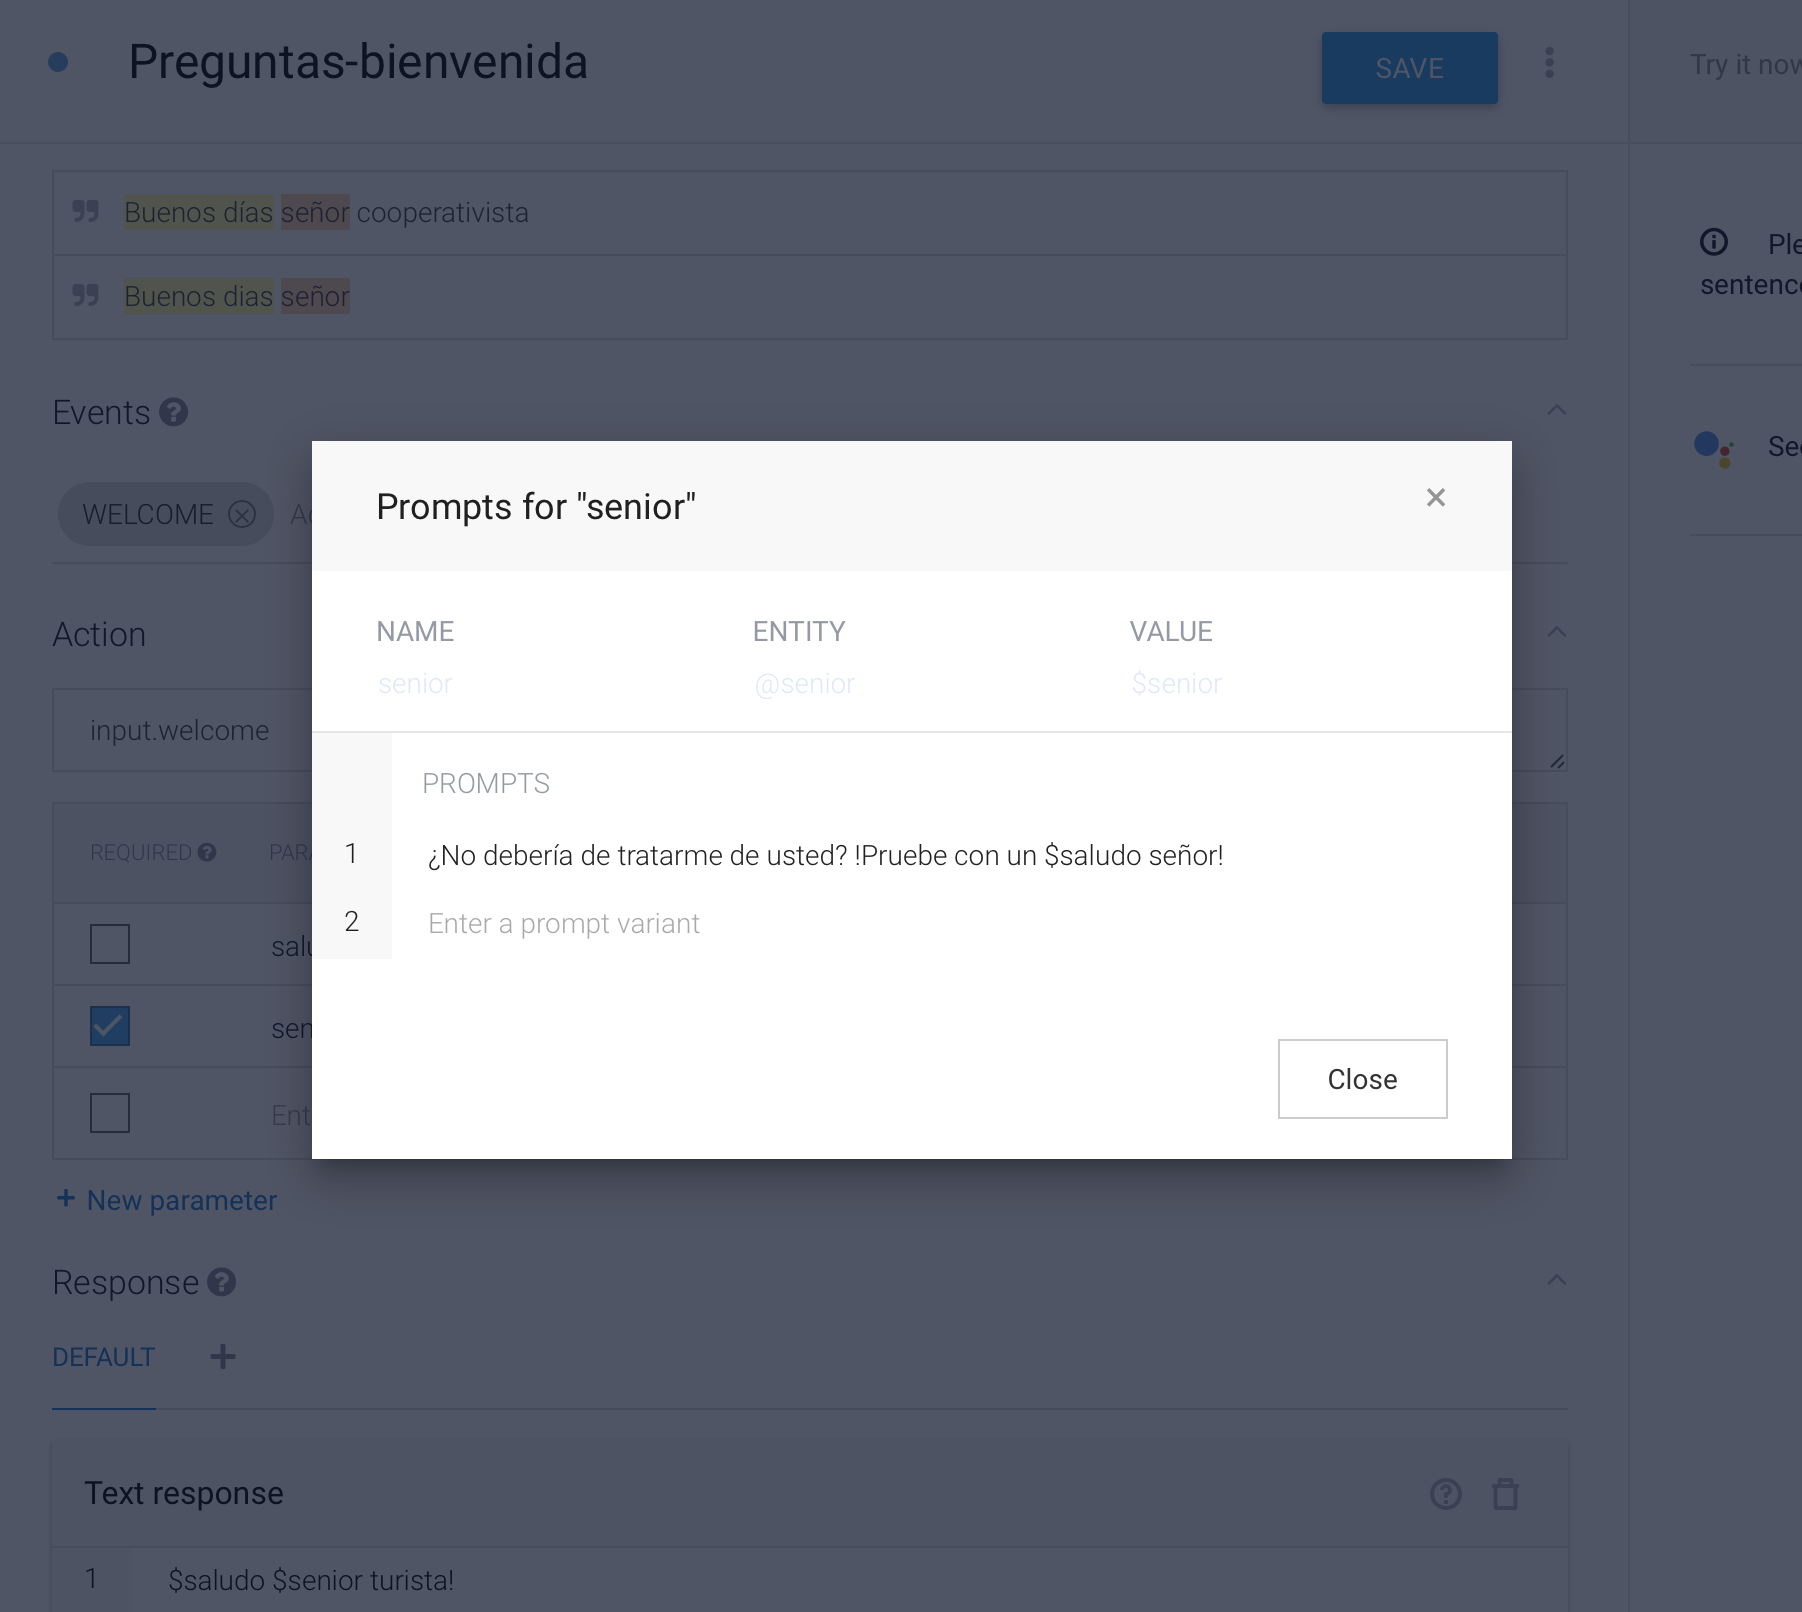
\includegraphics[scale=0.3]{imagenes/promts.png}  %el parámetro scale permite agrandar o achicar la imagen. En el nombre de archivo puede especificar directorios
	\caption{Ejemplo de uso de prompts}
\end{figure}


En caso de no saludar con este estilo el agente exigirá que le saludemos con educación. Este tipo de saludos ''informales'' serán almacenados en una entidad distinta llamada ''saludo-informal'', de modo que cuando detecte algún campo de estas entidades saltará un nuevo intento que nos pedirá que le saludemos con educación.


\subsubsection{Preguntas de información básicas}

Podremos preguntarle al personaje cosas como:
\begin{itemize}
	\item ¿Que tal?
	\item ¿Quién eres?
	\item ¿Qué preguntas puedo hacerle?
\end{itemize}
Cada una de estas preguntas se corresponden con diferentes ''Intents'' y cada uno responderá de manera diferente. Para estos tipos no hemos usado nada relevante a contextos, prompts o entidades.

\subsubsection{Preguntas relativas a la profesión del personaje}

Como nuestro personaje es un cooperativista del Valle de los Pedroches, podremos hacerle preguntas relativas a la cooperativa y su trabajo.\\ 

Dentro de este apartado tendremos preguntas encadenadas, que las hemos creado ayudándonos de los contextos y de las entidades.

\subsubsection{Cuando surgió}

Podemos preguntarle por ejemplo al personaje:
\begin{itemize}
	\item ¿Cuando nació la cooperativa?
	\item ¿En qué año surgió la cooperativa?
\end{itemize}
La respuesta del personaje será relativa a la fecha de cuando nació la cooperativa y preguntará al turista si desea saber como surgió la cooperativa. Entonces, emitirá un contexto de salida con un lifespan (esto es el tiempo de vida del contexto, es decir, el número de intentos durante el que estará activo el contexto). \\

\begin{figure}[H] %con el [H] le obligamos a situar aquí la figura
	\centering
	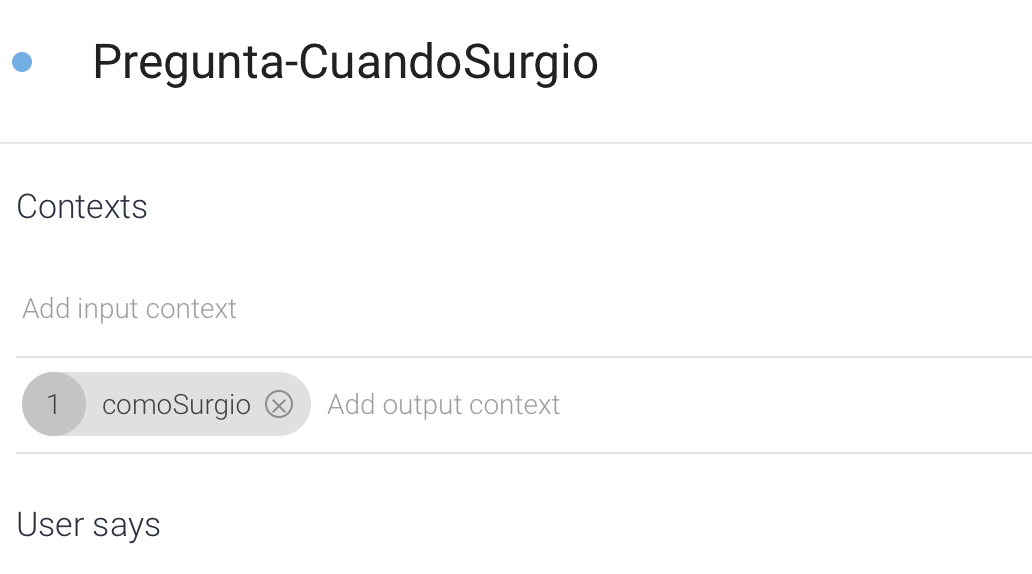
\includegraphics[scale=0.4]{imagenes/contextOut.png}  %el parámetro scale permite agrandar o achicar la imagen. En el nombre de archivo puede especificar directorios
	\caption{Ejemplo de uso de contexto de salida}
\end{figure}


De este modo, hemos creado un nuevo intento que tiene como contexto de entrada el contexto de salida de la pregunta anterior y que se activa cuando le decimos al personaje que sí queremos saber como surgió. El personaje entonces nos responderá con la respuesta adecuada. \\

\begin{figure}[H] %con el [H] le obligamos a situar aquí la figura
	\centering
	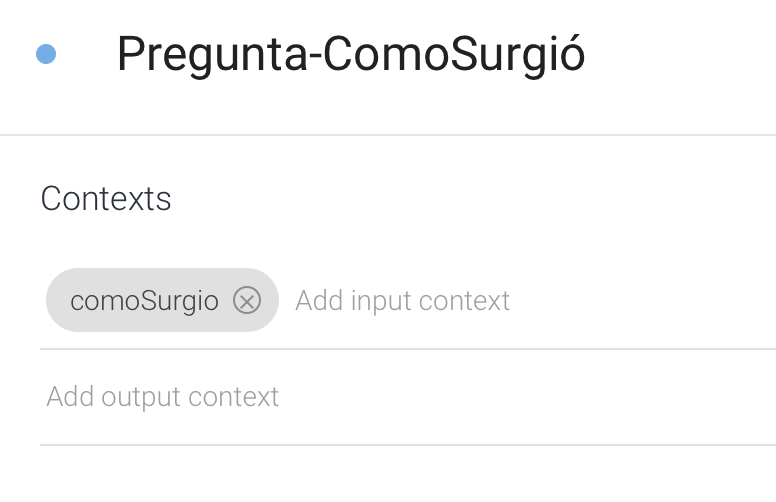
\includegraphics[scale=0.4]{imagenes/contextIn.png}  %el parámetro scale permite agrandar o achicar la imagen. En el nombre de archivo puede especificar directorios
	\caption{Ejemplo de uso de contexto de entrada}
\end{figure}
En caso de que no quiera conocer esa información, es decir, que respondamos no a la primera pregunta del agente, el personaje hará otra respuesta del tipo: ''Usted se lo pierde''. Hemos creado una entidad llamada ''no'' que incluye diversas respuestas negativas: que va, no, para nada ... etc. \\

Además, también se puede preguntar al personaje sobre como surgió la cooperativa aunque no hayamos preguntado antes el cuando, es decir, no encadenando las preguntas con contextos. Esto estará definido en un nuevo intento.


\subsubsection{Como han avanzado}
Podemos preguntarle al personaje:
\begin{itemize}
	\item ¿Cómo han llegado hasta ahora?
	\item ¿Cómo se organizaron para que esto llegara hasta aquí?
	\item ¿Cómo se han convertido en lo que es ahora?	
\end{itemize}

El agente responderá y nos dirá si deseamos saber que productos producimos. Al igual que antes este intento tendrá un contexto de salida que podrán recoger en caso de decir que si queremos que nos lo diga o en caso de que no queramos. \\

Podemos decir que sí, que tipo de productos hacen, que alimentos salen... y todas esas preguntas serán recogidas por el intent cuando exista el contexto anteriormente dicho y responderá con lo propio. Para el caso negativo responderá de forma similar al del apartado anterior. \\

Al igual que en el apartado anterior también podemos preguntar de forma que no haya ningún contexto activo por los productos que producen, para ello:

\begin{itemize}
	\item ¿Qué alimentos salen?
	\item ¿Qué tipo de alimentos producís?
\end{itemize} 

\subsubsection{Valoración}

Además de la conversación normal con nuestro agente, también podemos darle una valoración a unas determinadas preguntas que nos planteará el agente. Para ello empezaremos la valoración diciéndole: ''valorar''. Una vez hecho esto el agente nos hará una pregunta y nos pedirá una valoración para ella, de modo que en la siguiente pregunta que nosotros le hagamos le respondamos con una valoración u otra. Para recoger las valoraciones hemos usado una entidad denominada ''rate'', la cual tiene como tipos: excelente, buena, mala, regular. Para encadenar las preguntas hemos usado contextos. \\

Así pues, el agente nos planteará 3 preguntas y nos ofrecerá la posibilidad de recomendarnos a otros personajes relacionados con su profesión. No vamos a explicar pregunta por pregunta de la valoración ya que es exactamente que las anteriores pero usando contextos, además como hemos puesto de lifespan del contexto a 1, en caso de que no digamos una valoración correcta se saldrá de la valoración y tendremos que volver a empezar. 

\subsubsection{Despedida}
Una vez terminado podemos decirle adiós y el agente se despedirá diciéndonos que podemos darle una valoración también.


\subsubsection{Respuestas predeterminadas en caso de fallo en el reconocimiento}

En caso de que ninguna pregunta case con lo establecido o en caso de que no entienda lo que hemos dicho el agente nos responderá con las siguientes respuestas:

\begin{itemize}
	\item ¿Podría repetirlo, por favor?
	\item No estoy entendiendo que me pides. ¡Si no sabes que puedo hacer pregúnteme!
\end{itemize}

\subsubsection{Capturas de las entidades y los distintos intents}
%------------------------------------------------


\begin{figure}[H] %con el [H] le obligamos a situar aquí la figura
	\centering
	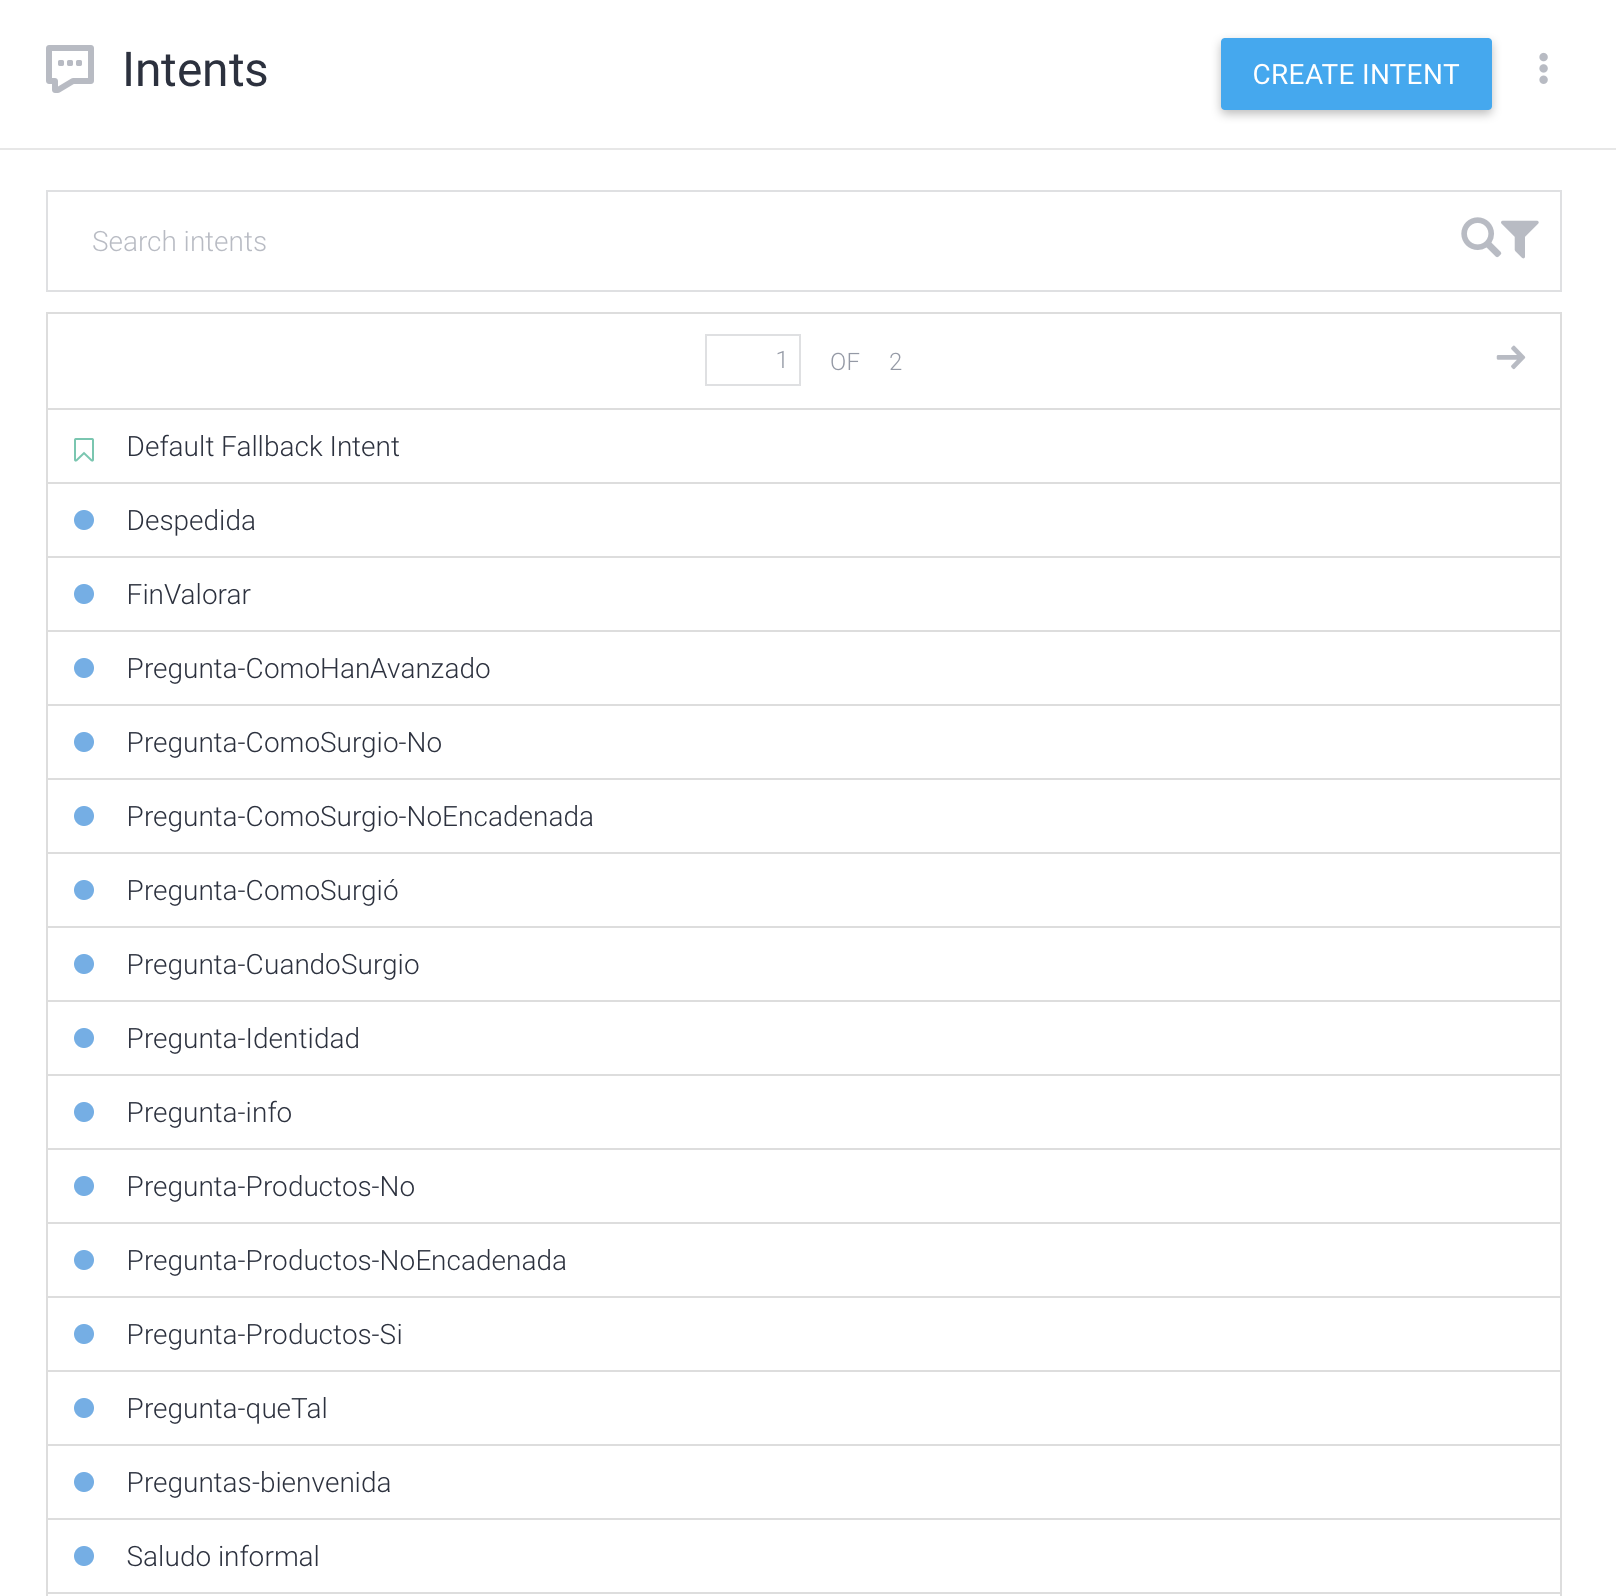
\includegraphics[scale=0.3]{imagenes/intents1.png}  %el parámetro scale permite agrandar o achicar la imagen. En el nombre de archivo puede especificar directorios
	\caption{Intents definidos (1)}
\end{figure}

\begin{figure}[H] %con el [H] le obligamos a situar aquí la figura
	\centering
	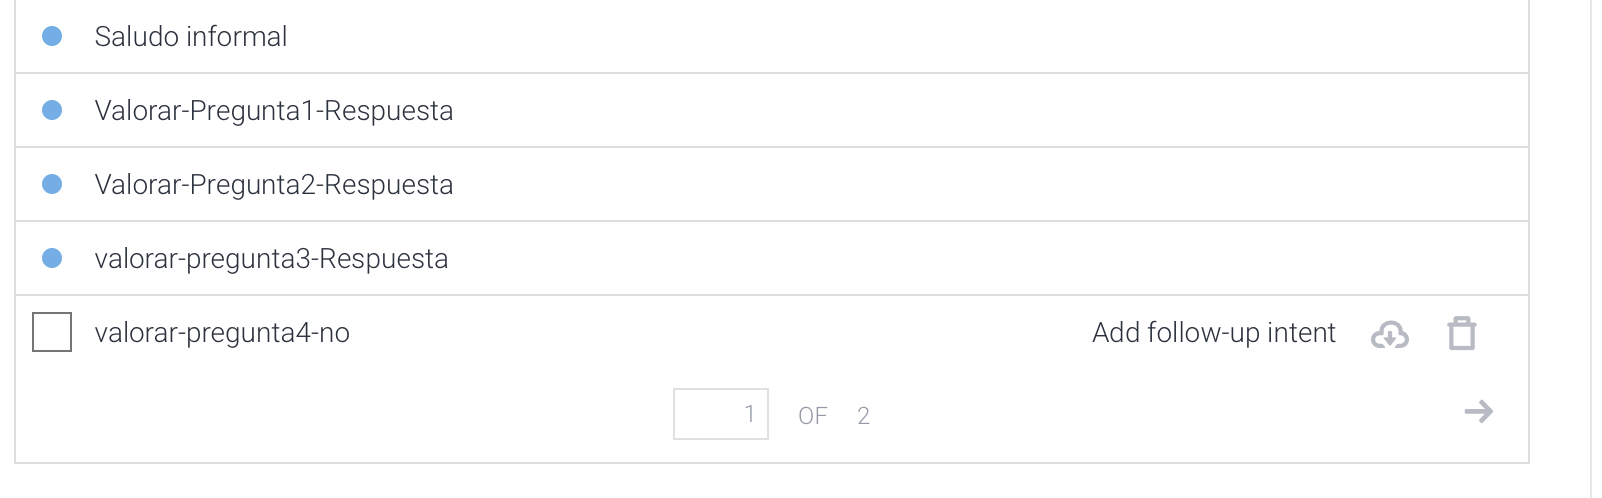
\includegraphics[scale=0.3]{imagenes/intents2.png}  %el parámetro scale permite agrandar o achicar la imagen. En el nombre de archivo puede especificar directorios
	\caption{Intents definidos (2)}
\end{figure}

\begin{figure}[H] %con el [H] le obligamos a situar aquí la figura
	\centering
	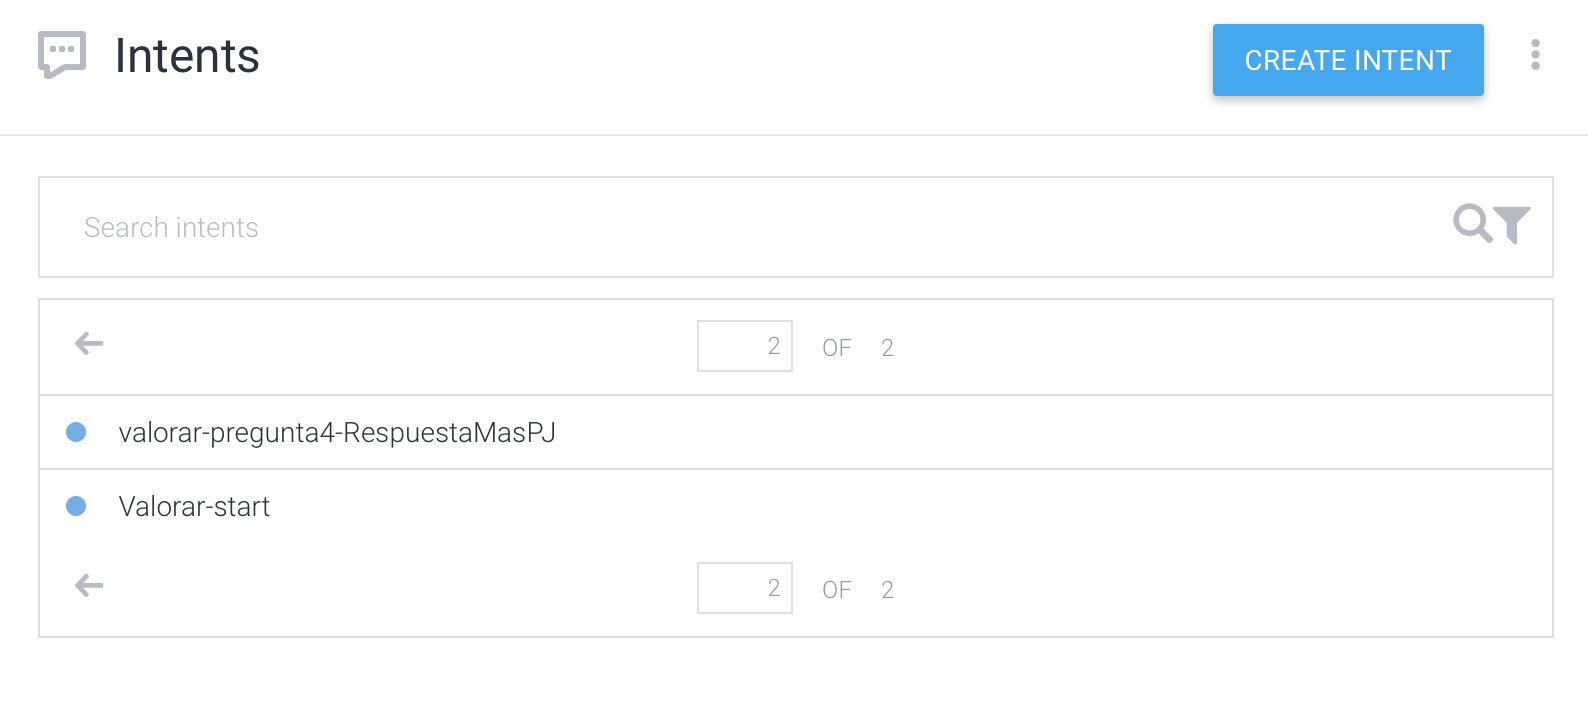
\includegraphics[scale=0.3]{imagenes/intents3.png}  %el parámetro scale permite agrandar o achicar la imagen. En el nombre de archivo puede especificar directorios
	\caption{Intents definidos (3)}
\end{figure}


\begin{figure}[H] %con el [H] le obligamos a situar aquí la figura
	\centering
	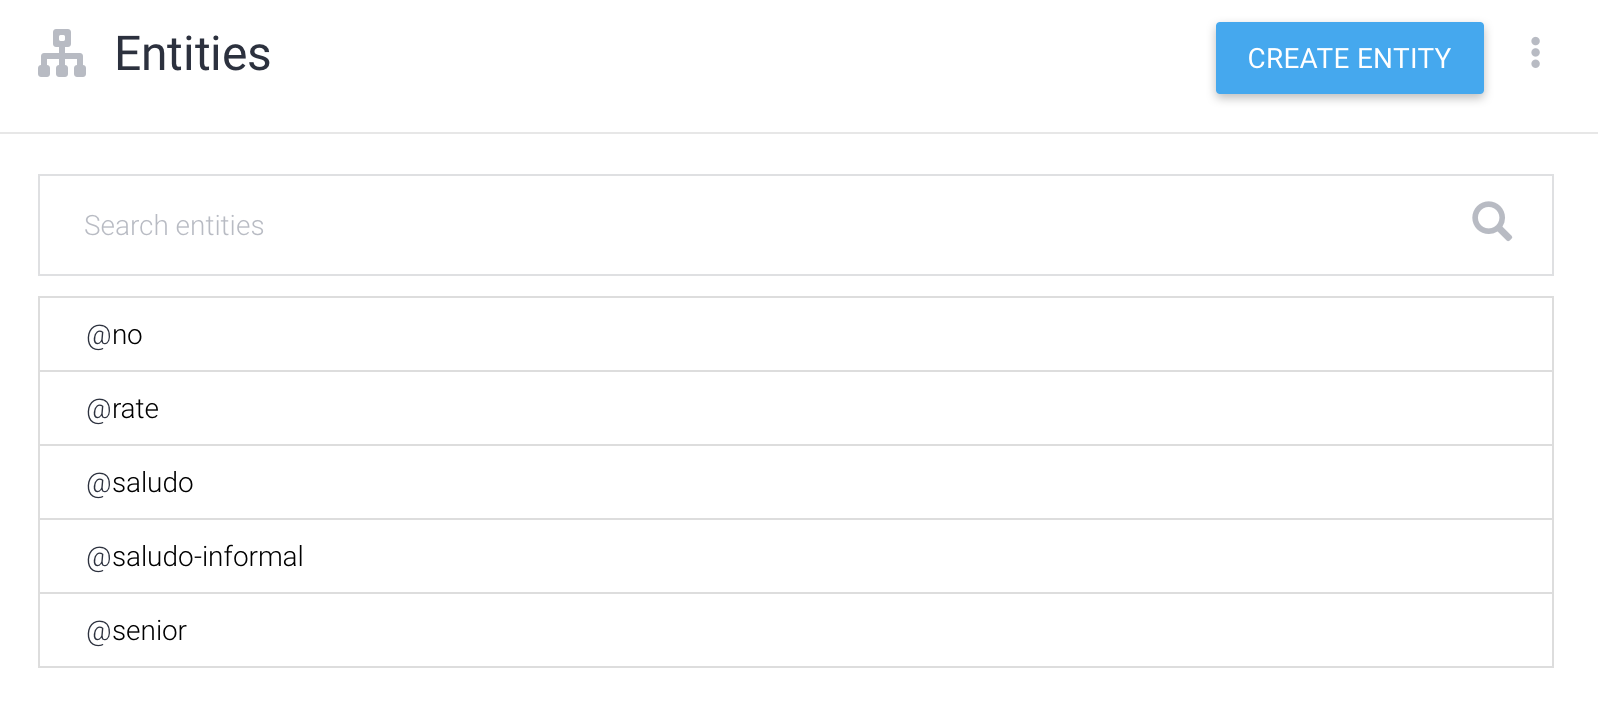
\includegraphics[scale=0.3]{imagenes/entidades.png}  %el parámetro scale permite agrandar o achicar la imagen. En el nombre de archivo puede especificar directorios
	\caption{Entidades definidas.}
\end{figure}


\subsection{Estructura y explicación de la implementación}
Para el desarrollo del código hemos empleado una mezcla entre el proyecto de Zoraida ''SimpleTTS'' y el proyecto explicado el github de dialogflow. \cite{git}
A continuación mostraremos la estructura de clases implementada en el código de la aplicación:

\begin{figure}[H] %con el [H] le obligamos a situar aquí la figura
	\centering
	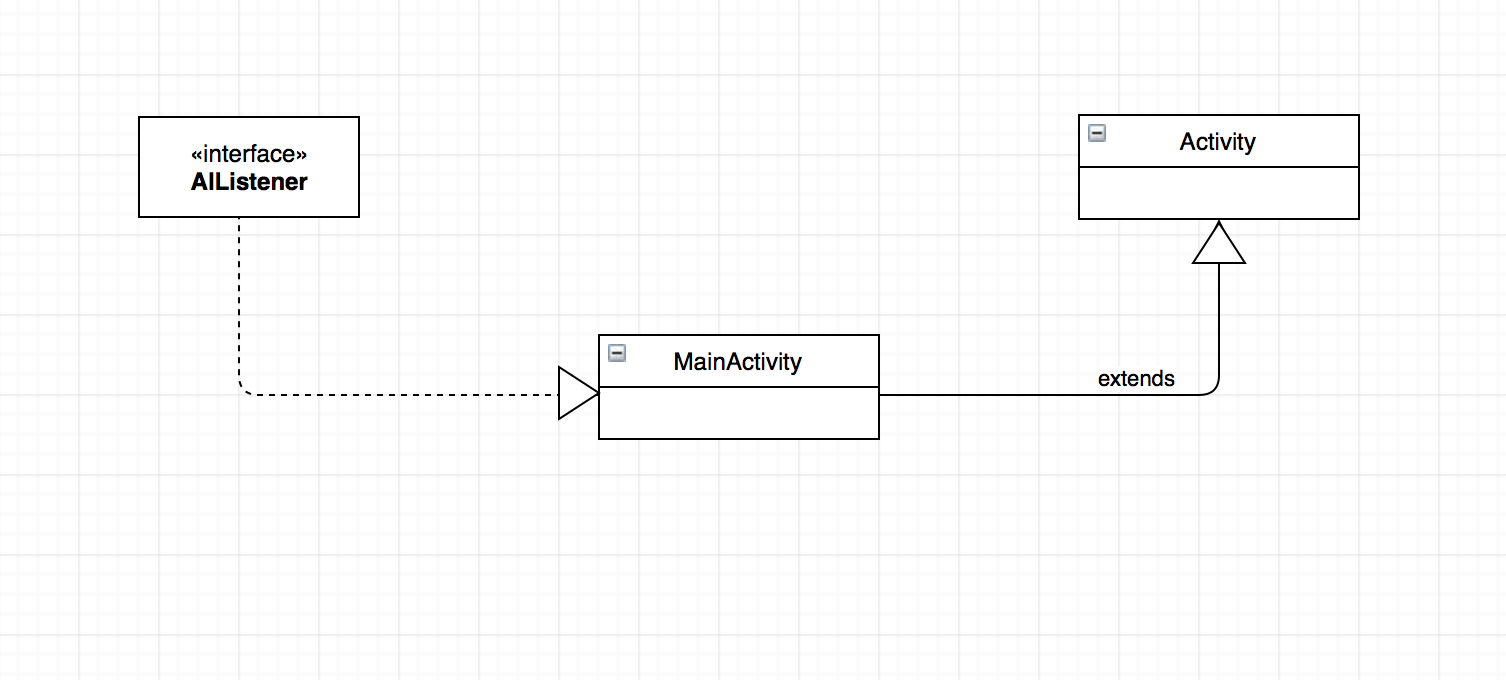
\includegraphics[scale=0.3]{imagenes/diagrama.png}  %el parámetro scale permite agrandar o achicar la imagen. En el nombre de archivo puede especificar directorios
	\caption{Entidades definidas.}
\end{figure}

\subsection{MainActivity} Es la clase principal, aquella que va a manejar la actividad del sistema. Hereda de la clase Activity e implementa la interfaz de escucha AIListener para el trabajo con el servicio API.AI. \\

En esta clase implementaremos y definiremos todo lo necesario para el reconocimiento de voz (preguntas), la comunicación con el procesador de lenguaje natural (DialogFlow) y la síntesis de voz (respuestas). Cabe destacar que la aplicación está implementada para ser compatible con la SDK 24 (Android 7) cómo mínimo y está compilada con la versión 25. Esto lo hemos decidido así ya que había problemas de compatibilidad con algunos elementos.\\

Una vez hemos añadido las bibliotecas necesarias, necesitamos agregar los siguientes permisos para conectarnos a internet y poder grabar audio:

\begin{itemize}
	\item android.permission.INTERNET 

	\item android.permission.RECORD\_AUDIO 
\end{itemize}

Una vez hecho esto comentaremos los datos miembros de relevancia, aunque en el código aparece todo bien explicado:

\begin{itemize}
	\item \textbf{aiService} Instancia del servicio que hará las solicitudes de consulta (AIService).
	\item \textbf{mytts:} Instancia del motor TextToSpeech que usaremos para sintetizar el texto obtenido del agente de DialogFlow.
	\item \textbf{idiomaActivo:} String que nos indicará el idioma activo tanto de sintentización como de reconocimiento de audio.
	\item \textbf{dialogEN:} Token de acceso al agente de dialog flow español.
	\item \textbf{dialogES:} Token de acceso al agente de dialog flow inglés.
\end{itemize}
Los demás atributos se especifican y explican en el código.
\newpage

Una vez explicado esto pasaremos a la inicialización. Para ello hemos sobre escribiendo la función onCreate, donde destacaremos las cosas relevantes: 
\begin{itemize}
	\item Creamos una instancia de AIConfiguration para indicar que agente se usará para el procesamiento del lenguaje e indicaremos el token de acceso del cliente, el lenguaje que soporta (inicialmente será español) y le indicaremos que usará el motor de reconocimiento del sistema.
	\item Utilizamos la instancia de AIConfiguration creada anteriormente para obtener un objeto que haga referencia al AIService, que será el que haga las solicitudes de consulta.
	\item Establecemos la instancia de AIListener para la instancia de AIService.
	\item Iniciamos el motor de síntesis TTS, con las comprobaciones necesarias (initTTS).
\end{itemize}

De lo mencionado anteriormente cabe ampliar la definición de la función \textbf{initTTS}. Esta función inicia la comprobación para saber si el motor de síntesis de voz está o no instalado. Cuando termina llama al método \textbf{onActivityResult} automáticamente. Cuando comprobamos si el motor de síntesis está instalado se llama automáticamente a la función onActivityResult, que la sobre escribiremos, y en caso de estar instalado crearemos una instancia de TextToSpeech (inicializamos mytts) para realizar síntesis de audio. Si no está instalado, creará un intento para instalar el motor de TexToSpeech. Cabe destacar que  inicializaremos el motor tts con lenguaje español. \\

Ahora podemos hacer una descripción de los elementos relevantes de la pantalla inicial, donde tenemos:

\begin{itemize}
	\item Una imagen del personaje que será el botón ( 
	imagenPersonaje, de la clase ImageButton) con el que inicializaremos la grabación de audio.
	\item Un campo de texto (resultTextView) donde imprimiremos la respuesta del agente a la última pregunta del turista.
	\item Una bandera, que será un botón (imagenBandera, de la clase ImageButton) que indicará el idioma actual de síntesis y reconocimiento.
\end{itemize}

\begin{figure}[H] %con el [H] le obligamos a situar aquí la figura
	\centering
	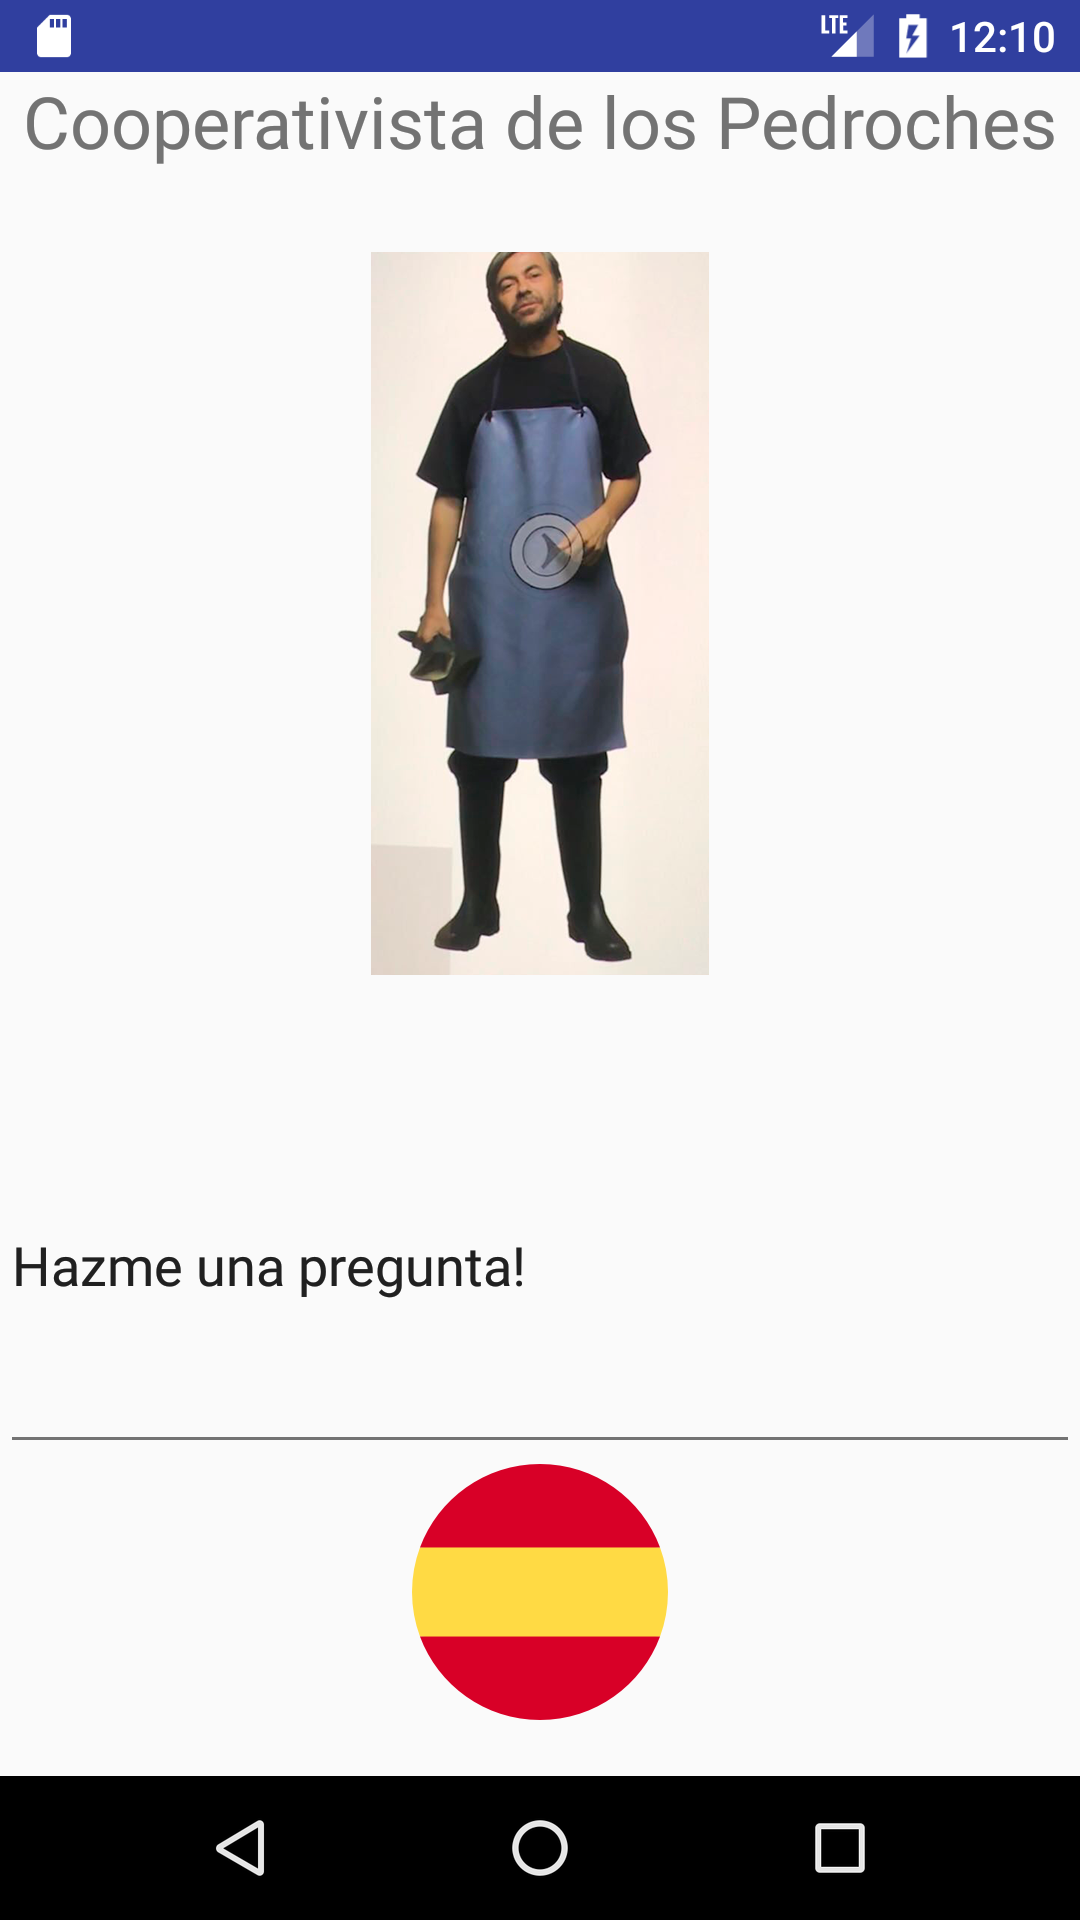
\includegraphics[scale=0.2]{imagenes/app_oral.png}  %el parámetro scale permite agrandar o achicar la imagen. En el nombre de archivo puede especificar directorios
	\caption{Captura de pantalla de la aplicación de interfaz oral.}
\end{figure}
Al pulsar el botón del personaje vamos a intentar iniciar el reconocimiento de voz ( se lanzará automáticamente la función \textbf{listenButtonOnClick}), para ello en primer lugar vamos a comprobar que tenemos conexión a Internet, ya que si no no podremos conectarnos con el servidor de DialogFlow y por tanto mostraremos un mensaje diciendo que no estamos conectados a internet y no iniciaremos la escucha. \\ 

Para ello hemos usado una función llamada estaConectado ayudándonos de la página referenciada en la documentación del código, aunque esta función sólo nos dice si estamos conectados a la red pero no comprueba que tenemos conexión luego si estamos ante redes privadas donde necesitamos poner un usuario y contraseña y no la tengamos introducida (como ciugr) aunque nos diga que tenemos conexión no podremos conectarnos a DialogFlow. Para solucionar esto podemos añadir al código hacer ping a servidores como Google o Facebook que sabemos que no se van a caer con facilidad para comprobar esto. \\

Una vez hemos comprobado la conexión a internet, procederemos a comprobar los permisos de grabación de audio antes de empezar a escuchar. \\

Se llamará a la función \textbf{checkPermission} y posteriormente a la función \textbf{onRequestPermissionsResult} cuando se complete la llamada a la función anterior, ambas sacadas del proyecto ''simpleTTS'', las cuales pedirán al usuario que se le otorge a la aplicación permisos de grabación de audio ya que si no no se puede continuar. \\

Una vez comprobado esto iniciaremos la escucha mediante la llamada a la función \textbf{aiService.startListening()}. Cuando el reconocimiento finalice, si no hay errores, se activará la función \textbf{onResult}. Esta función obtendrá todos los campos devueltos por el agente tras completar la solicitud, extrayendo de estos la respuesta para mostrarla en el campo de texto (resultTextView). Una vez hecho esto llamamos a la función \textbf{Synthesized}, que se encargará de sintetizar usando mytts.speak la respuesta que hemos introducido en el campo de texto. \\

En caso de errores del tipo que no haya resultados para la pregunta o errores al escuchar, devolveremos en el campo de texto el mensaje: "No he escuchado nada o no hay resultados para su pregunta" para que el usuario sepa que ha habido un error y pueda volver a repetir la pregunta. Dentro de esto se puede tratar diversos tipos de errores y almacenarlos en logs y demás para corregirlos posteriormente, pero ya que era un prototipo no hemos querido ir más allá. \\ 

Ahora vamos a hablar del botón de la bandera, el botón que nos proporcionará el cambio de idioma, de modo que si estamos en español cambiará a inglés y si estamos en inglés cambiará a español. Para ello en primer lugar crearemos una nueva instancia de AIConfiguration con el token (dialogEN o dialogES) correspondiente al agente de DialogFlow en Español o en Inglés, depende de al que queramos cambiar. Posteriormente repetimos el proceso anterior realizado en la inicialización, menos la llamada al initTTS. Una vez hecho esto, solo nos faltará cambiar el idioma al sintetizador de audio (mytts), para ello comprobamos si está disponible y usamos \textbf{mytts.setLanguage}.\\


Por último cabe destacar que hemos bloqueado los botones de escuchar y de cambiar de idioma cuando se haya pulsado ya el botón de escucha para que no podamos usarlos hasta que se termine de escuchar una pregunta. También, cuando estemos sintetizando una respuesta, si hemos pulsado de nuevo el botón de escuchar o el botón de cambio de idioma vamos a parar automáticamente la síntesis de respuesta para que el comportamiento sea más real y podamos detener al agente. Obviamente, cuando se pasen todas estas situaciones se desbloquean los botones. Para ello usamos las funciones: \textbf{disableSpeakButton} y \textbf{enableSpeakButton}. \\

La parte relativa a la interfaz oral ha sido realizada por \textbf{Juan Ramón Gómez Berzosa}.

\section{Interfaz sensorial por móvil}
Primeramente explicamos la idea de funcionamiento de cada uno de los sensores implementados a la hora de ejecutar la aplicación.
\subsection{NFC}
Una vez nos ambientamos en la época, como hemos mencionado antes, se mostrarán en las estructuras del museo distintos puestos de un mercado de la época y vitrinas con etiquetas NFC identificativas a través de las cuales, utilizando el lector NFC de nuestro dispositivo móvil, tendremos acceso a fotos descriptivas e información asociados a la etiqueta correspondiente. Por ejemplo, en nuestro mercado virtual de cierta época puede existir un puesto dedicado a la comida, en dicho puesto puede haber una serie de etiquetas repartidas por la mesa, cada una de las cuales haga referencia a un tipo de comida distinto; a la hora de escanear con mi dispositivo móvil una de las etiquetas en el apartado correspondiente de la aplicación del museo, aparecerá en la pantalla del dispositivo una serie de imágenes del alimento asociadas a la etiqueta, así como información de referencia acerca de este.\\
De esta misma forma serán tratadas las vitrinas que haya repartidas por el museo, es decir, con etiquetas NFC que nos proporcionen la 'llave' para acceder a la información desde nuestro dispositivo móvil.

\subsection{Acelerómetro}
Una vez haya detectado una etiqueta NFC nuestro dispositivo, se nos proporcionará acceso a cierta información: imágenes, texto, vídeo, etc. Como toda esa información asociada a una misma etiqueta no cabe en la pantalla de
un dispositivo normal, hemos implementado un cambio entre pantallas de la información de una etiqueta a través del acelerómetro existente en el dispositivo móvil, es decir, si escaneamos una etiqueta NFC con el móvil y de primera mano nos aparece la foto de unas especias típicas de la época (por ejemplo), con tan solo agitar el dispositivo, la foto se cambiará por otra foto asociada a esa etiqueta, por un texto descriptivo de la imagen, etc.

\subsection{GPS}

La idea de la aplicación es que solo pueda ser utilizada en el museo para el que fue creada. Con este objetivo, mediante el sensor GPS (sistema de posicionamiento global), se ha introducido la limitación al usuario de poder utilizar las funciones de la aplicación únicamente cuando esté dentro del museo. Esto se ha hecho especificando a la aplicación un rango de actuación en términos de latitud y longitud. Si el usuario se encuentra fuera del rango dado, aparecerá un mensaje en la aplicación informándole de la imposibilidad de ser utilizada.

\subsection{Interacción táctil}

Con el fin de adentrarnos más en la experiencia, en uno de los apartados de la aplicación, el usuario tendrá acceso a un mapa del museo donde podrá orientarse por la sala, sabiendo donde está la zona de interacción oral, la zona del mercado, la zona de exposición de armas, etc.

\subsection{Estructura y explicación de la implementación}

A continuación mostramos la estructura de clases implementada en el código de la aplicación:

\begin{figure}[H]
	\centering
	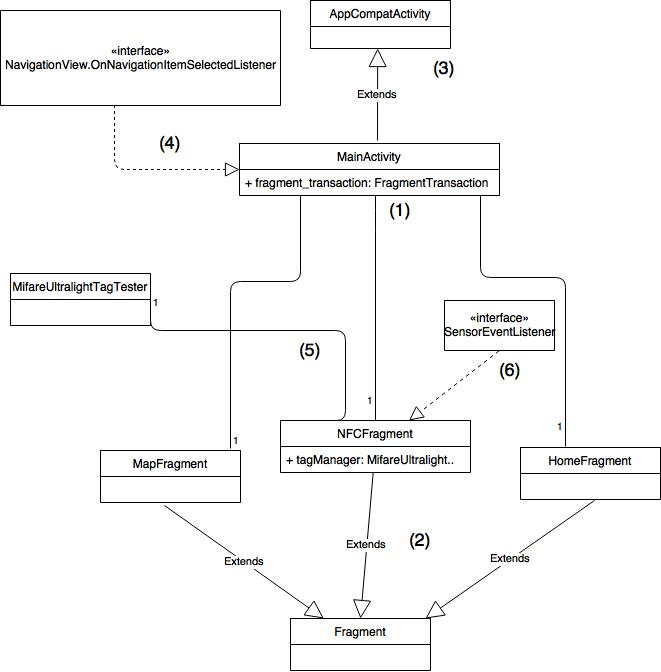
\includegraphics[width=0.85\textwidth]{imagenes/diagrama.jpg}
	\caption{Diagrama de clases implementado.}
\end{figure}

\begin{enumerate}
	\item \textbf{Main Activity}: se trata de la clase principal, aquella que lleva la actividad ('activity'), es por eso que hereda el comportamiento de \textit{AppCompatActivity} (3). \textit{Main Activity} se encarga de detectar si el usuario se encuentra dentro del museo para entonces, y solo entonces, habilitar las demás funcionalidades al usuario (escaneo de NFC, mapa...) para que este pueda lanzarlas, acción que también es llevada a cabo por esta misma clase. Además, es la encargada de llevar el intercambio en la vista relacionandose con cada \textit{Fragment} correspondiente (1). A continuación describimos de forma breve las funciones más importantes que posibilitan dicho comportamiento:
		\begin{itemize}
			\item \textbf{CheckLocationPermission}: se encarga de comprobar si el teléfono tiene permisos para el uso del sensor GPS.
			\item \textbf{onRequestPermissionResult}: recibe la información analizada por la función anterior y, en caso de que haya permisos para el uso de GPS, le pide al gestor de localización del dispositivo, la localización actual de este.
			\item \textbf{CheckLocation}: usando la localización proporcionada por la función anterior, comprueba si el dispositivo se encuentra dentro del rango predefinido por la aplicación, en cuyo caso activará el uso de todas las funcionalidades.
			\item \textbf{onNavigationItemSelected}: una vez la aplicación sabe que estamos dentro del museo, podremos desplegar la barra lateral de herramientas para seleccionar un item, una funcionalidad, cuya vista reemplazará a la actual en la interfaz (esta acción es tratada en esta misma función).
		\end{itemize}
	\item \textbf{NFC Fragment}: Esta clase la cuál hereda comportamiento de Fragment (2), se ocupa de la detección y tratamiento de las etiquetas NFC repartidas por todo el museo así como la interacción con la información que estas proporcionan mediante el acelerómetro. Primeramente se ocupa de activar el uso del sistema de detección de etiquetas y más tarde de detectar la etiqueta escaneada para dar acceso al usuario a una información u otra. Para escuchar y tratar los eventos correspondientes con dichos sensores es necesario que implemente la interfaz \textit{SensorEventListener} (6). Una vez proporciona acceso a dicha información, la clase estará pendiente de los movimientos que haga el usuario con la mano para, mediante el acelerómetro, realizar el cambio en pantalla de la información actual (una imagen) por otro tipo de información (descripción de la imagen) y viceversa. A continuación describimos de forma breve las funciones más importantes que posibilitan dicho comportamiento:
		\begin{itemize}
			\item \textbf{enableReaderMode}: función que activa el modo lectura en el sensor de escaneo NFC.
			\item \textbf{onTagDiscovered}: se encarga de tratar el escaneo de la etiqueta NFC mediante la comunicación con el objeto \textit{tag\_manager} obtenido de la relación (5). Recibe la etiqueta escaneada y, dependiendo del identificador que tenga, proporciona al usuario una imagen u otra. En la actual aplicación si la etiqueta tiene como identificador el valor '1', se muestra una foto de una paella, si tiene como identificador el valor '2', se mostrará una imagen de una serie de especias.
			\item \textbf{detectShake}: en caso de que el usuario agite el teléfono y tenga en su pantalla una imagen, o un texto asociados a una etiqueta NFC, esta función se encargará de comprobar si la fuerza realizada por el usuario al agitar el teléfono es suficientemente grande, en cuyo caso, el elemento activo en pantalla cambiará a otro elemento asociado a la misma etiqueta NFC (esta acción es tratada dentro de esta misma función, es decir, se comprueba el elemento activo en pantalla para proporcionar otro tipo de información relativa a dicho elemento)
		\end{itemize}
	
	
	\item \textbf{MiFareUltralightTagTester}: Dicha clase es la que posee el comportamiento a más bajo nivel para establecer la comunicación con la tecnologia NFC detectada (tag). Una vez obtenido un \textit{tag} NFC con el que establecer la comunicación, mediante dicha clase podemos realizar las tareas I/O con dicha etiqueta y nuestro dispositivo móvil. 
	A continuación describimos de forma breve las funciones más importantes que posibilitan dicho comportamiento:
	
	\begin{itemize}
		\item \textbf{writeTag}: Dado un tag NFC, permite escribir información en dicho tag. Util para la configuración inicial de los tag, permitiendo definir un nombre a cada acción correspondiente en nuestra aplicación.
		\item \textbf{readTag}: Nos permite obtener en formato texto el contenido de la etiqueta NFC detectada. En función del contenido nuestra aplicación se encargará de realizar las acciones oportunas.
	\end{itemize}



	\item \textbf{Map Fragment}:  Esta clase contiene la implementación del comportamiento del subapartado correspondiente al mapa de nuestro museo. En ella se habilitan ciertas acciones y gestos sobre la pantalla táctil de forma que la interacción del usuario con el mismo sea mucho más flexible y útil. A grandes rasgos, permite realizar un \textbf{escalado} o \textbf{zoom} del mapa hasta un nivel de detalle determinado (proporción máxima 3.5 veces la escala inicial), además de habilitar el desplazamiento de la vista del mapa en cualquier dirección de la pantalla. Como funcionalidades adicionales, se le permite al usuario hacer uso de un \textbf{doble tap} sobre la pantalla para aumentar la vista un 50\% y reescalar el mapa a su tamaño inicial con sólo mantener pulsado la pantalla durante un muy breve periodo de tiempo. Por último, se describen aquellas clases y funciones que hacen posible el funcionamiento de este apartado.
	
	\begin{itemize}
		\item \textbf{onCreateView}: crea un objeto de vista (View) del fragmento, al cual se le asocian dos objetos, cada uno de una clase distinta, que permitirán capturar los eventos de tipo \textit{zoom} y aquellos más generales, como el \textit{double tap} o el \textit{Long Press}. Estos dos tipos de eventos serán escuchados por un método \textbf{onTouch}, que se activa cada vez que ocurre un evento de tipo táctil sobre la pantalla, y en función del número de dedos, pasará el control a uno de los dos objetos que describimos a continuación:
		\begin{enumerate}
			
			\item \textbf{Clase ScaleListener}: hereda comportamiento de la clase \textbf{ScaleGestureDetector.SimpleOnScaleGestureListener} permitiendo que el método \textbf{onScale} detecte los eventos de tipo escalado y que realice el mismo siempre y cuando se cumplan ciertas condiciones. La escala se puede modificar siempre y cuando esté dentro de un valor mínimo (escala 1:1) y un valor máximo (escala 3.5).

			La función \textbf{escalarVista}, que es llamada dentro de \textbf{onScale} para realizar el escalado, recibe un punto (X,Y) que actuará de centro para el escalado (el punto medio de ambos dedos sobre la pantalla) así como la escala que se quiere aplicar a la vista del mapa.	
			
			\item \textbf{Clase MyGestureListener}[BIB]: mediante la herencia del comportamiento de la clase \textbf{GestureDetector.SimpleOnGestureListener} permite a la clase principal escuchar eventos de tipo \textbf{Gesture} en la pantalla táctil, sobreescribiendo la definición de los métodos que detectan a cada uno prestando especial atención a los 3 siguientes:
			
			\begin{itemize}
				\item \textbf{onScroll}: realiza el desplazamiento efectivo de la vista del mapa en función del movimiento del dedo sobre la pantalla.
				
				\item \textbf{onDoubleTap}: permite realizar un escalado dinámico a un 50\% más de la escala actual.
				
				\item \textbf{onLongPress}: al detectar presión continuada durante un breve periodo de tiempo, recupera la vista original a su escala 1:1.
			\end{itemize}

		\end{enumerate}
	\end{itemize}

	
	
	
	
\end{enumerate}


La parte relativa a la interfaz sensorial ha sido realizada por \textbf{Samuel Cardene Rodríguez} y \textbf{Carlos Manuel Sequí Sánchez}, a excepción de la parte del mapa (sensor multitouch) que ha sido realizada por \textbf{Arthur Mickael Rodríguez Nesterenko}.

\newpage 
\subsection{Interfaz Gestual}

La interacción con los elementos del museo será mucho más versátil, dinámica y divertida para el usuario si hacemos uso de una interfaz gestual, que no es más que la \textbf{utilización de un dispositivo de detección del movimiento de nuestro cuerpo para permitirnos interactuar con elementos virtuales del museo}. En este caso en concreto se ha utilizado el dispositivo conocido como \textbf{Leap Motion}, el cual es capaz de detectar los movimientos y gestos de nuestras manos para que seamos capaces de realizar acciones directamente dentro de la interfaz virtual del museo. 
\\

¿Que interacción permite esta interfaz dentro de nuestro museo? La idea principal pasa por utilizar este dispositivo para permitir al usuario la navegación e interacción a través de una \textbf{amplia gama de herramientas, armas y/o armaduras de la época} donde se ambienta el museo, de forma que el visitante pueda seleccionar el objeto que desee consultar realizando \textbf{simples gestos con la mano} y que una vez seleccionado el mismo se le permita navegar a través de su estructura utilizando otra vez las manos, como si se tratase de un modelo real que el usuario pudiese estar tocando, permitiendo ver el objeto desde cualquier punto de vista que el usuario sea capaz de conseguir mediante el movimiento de sus manos e incluso acercar y alejar la vista del objeto para conseguir el máximo realismo posible, añadiendo además información relevante sobre las características del objeto en cuestión.\\

Esta interfaz gestual estará ligada directamente a una pantalla de tamaño determinado donde se proyectará el contenido virtual del objeto, pudiendo además ajustar la posición del dispositivo de detección de gestos a gusto o necesidad del usuario del museo, pensando en ofrecer una experiencia de la más alta calidad posible a cualquier persona, incluso si ésta posee alguna discapacidad psicomotora. Para ello, los dispositivos se encontrarán en pequeñas cajas que el usuario podrá colocar en apoyos cercanos a la pantalla (a distintas alturas) o incluso en los reposabrazos de las sillas de ruedas, sin alterar en ningún momento la capacidad de interacción.

\subsubsection{Estructura y explicación de la implementación}

Para hacer posible la implementación de esta interfaz se ha utilizado el Software Development Kit del dispositivo Leap Motion, creando un prototipo de interfaz de usuario que incluye las principales funcionalidades descritas con anterioridad. La estructura de clases se muestra a continuación y posteriormente se procederá a la explicación en mayor o menor medida segun se requiera.

\begin{figure}[H]
	\centering
	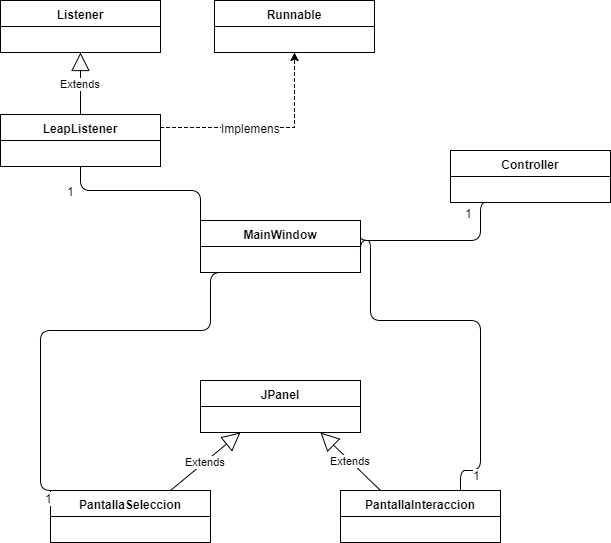
\includegraphics[width=0.85\textwidth]{imagenes/InterfazGestual}
	\caption{Diagrama de clases de la interfaz gestual.}
\end{figure}

Si bien la representación de las clases es sencilla, el funcionamiento y la interaccion entre clases es un poco complejo, por lo que a continuación explicaremos el contenido y la labor de cada clase y como se relaciona con las demás.

\begin{itemize}
	\item \textbf{Clase LeapListener}: es la clase que \textbf{gestiona todos los eventos relacionados con el sensor Leap Motion}. A través de esta clase, que se ejecuta en una hebra separada (pero hija de la clase principal) para no interferir con el funcionamiento de la interfaz, somos capaces de detectar cuando el dispositivo \textbf{cambia de estado}, concretamente entre disponible, conectado, desconectado y no disponible. Además de eso, guardamos información relacionada con los\textbf{ dos últimos frames} (paquetes de datos) recibidos, así como \textbf{cualquier gesto nativo detectado y su tipo}. 
	
	La función mas importante de ésta clase es \textbf{onFrame} que se ejecuta cada vez que el dispositivo envía un paquete de datos, actualizando los valores de la información detallada anteriormente. También se implementa la función \textbf{run} que permite ejecutar en una hebra separada.
	
	\item \textbf{Clase MainWindow}: es la clase principal del programa, aquella que controla el flujo de comunicación y ejecución dentro del mismo. Guarda información relacionada con el sensor (clases \textbf{Controller} y \textbf{LeapListener}) así como de las distintas pantallas de ejecución. A continuación se describen los métodos más importantes de la misma.
	
		\begin{enumerate}
			\item \textbf{Constructor de la clase}: lo más importante es destacar la creación de una hebra hija de esta clase que ejecutará todo lo relacionado con la clase \textbf{LeapListener}, gestionando la recepción de eventos y la actualización de la información correspondiente con este objeto.
			
			\item \textbf{addComponentToPane}: añade dos paneles de contenido; concretamente dos objetos, uno de la clase \textbf{PantallaSeleccion} y otro de la clase \textbf{PantallaInteraccion}. Estas dos clases se describirán más adelante.
			
			\item \textbf{gestionDeAplicacion}: es el método principal. Permite la interacción con el sensor de la siguiente manera: mientras la mano esté colocada sobre el rango del sensor, se podra interactuar con la interfaz. Pasados 1 segundo sin detección de la mano, pasa a modo reposo, esperando que el usuario vuelva a colocar la mano sobre el sensor. 
			
			Una vez detectada la mano el siguiente paso es detectar los gestos que me permiten moverme a través de las distintas pantallas. Se puede pasar de esta pantalla a la pantalla de selección de armas/herramientas haciendo un gesto circular con un dedo en el sentido de las agujas del reloj. En la pantalla de selección, realizando un barrido con la mano hacia la izquierda o derecha nos desplazamos por los distintos objetos y cerrando el puño seleccionaremos uno en concreto, pasando a ejecutarse la pantalla de interacción donde moveremos nuestra mano para interactuar con el objeto, pudiendo volver a la pantalla de selección realizando un giro circular de un dedo en sentido antihorario.
		\end{enumerate}	
	
		La ejecución de esta última función se realiza cada 200ms para evitar sobrecargar el sistema de información innecesaria.
	
	\item \textbf{Clase PantallaSeleccion}: posee información relacionada con los datos actualizados que envía el dispositivo, así como de la acción que deberá realizar el controlador (Clase MainWindow) en función de los gestos del usuario. Explicamos los métodos a continuación:
		\begin{enumerate}
			\item \textbf{detectarSentidoGiro}: nos dice si el sentido de giro de un Gesture de tipo CIRCLE es en sentido horario o antihorario.
			
			\item \textbf{detectarDireccionSwipe}: indica si el Gesture de tipo SWIPE se ha realizado hacia de izquierda a derecha o viceversa.
			
			\item \textbf{comprobarGrab}: detecta si la mano del usuario está lo suficientemente cerrada (un 90\%) como para considerarlo un gesto voluntario o no.
			
			\item \textbf{gestionarPrimeraPantalla}: traduce los gestos del usuario en acciones a realizar sobre la primera pantalla. Si el usuario realiza un barrido con la mano, se cambiará la vista del posible objeto que puede seleccionar, realizando esta selección cuando cierre de forma voluntaria la mano un 90\% (gesto Grab).
		\end{enumerate}
	
	\item \textbf{Clase PantallaInteraccion}: gestiona los eventos y las acciones del usuario una vez ha seleccionado el modelo con el que quiere interactuar a través de gestos. En esta pantalla el usuario podrá desplazar la mano horizontalmente para tener una vista de 360º del objeto seleccionado, así como aumentar la vista del mismo, realizando un zoom acercando o alejando la mano del dispositivo. 
	
	Todas estas acciones están controladas por un método \textbf{gestionarPantallaInteraccion} que decide que acción realizar en función de los gestos que realiza el usuario. Como bien se comentaba antes, se le da la oportunidad al usuario de volver a la pantalla anterior para seleccionar otro objeto distinto con tan solo girar un dedo en sentido antihorario.
	\end{itemize}

La parte relativa a la interfaz sensorial ha sido realizada por \textbf{Arthur Mickael Rodríguez Nesterenko}.
\newpage

\bibliography{citas} %archivo citas.bib que contiene las entradas 
\bibliographystyle{plain} % hay varias formas de citar

%----------------------------------------------- -



\end{document}
